%-----------------------------------------------------------------------------------------------------
%% fei --- classe para apresentações da equipe robofei
%% Author: Marcos Laureano
%% E-mail: marcos.laureano@ifpr.edu.br
%% 
%% Released under the LaTeX Project Public License v1.3c or later
%% See http://www.latex-project.org/lppl.txt
%% -----------------------------------------------------------------------------------------------------


\documentclass[xcolor=svgnames,8pt]{beamer} 

\usepackage{palatino}

\usepackage{verbatim}
\usepackage{graphicx,url}
\usepackage[brazil]{babel}   %mude aqui se desejar
\usepackage[utf8]{inputenc} 
\usepackage[T1]{fontenc} 
\usepackage{mathtools}
\usepackage{amsmath}
\usepackage{amssymb}
\usepackage{fontawesome}
\usepackage{booktabs}

\usepackage{adjustbox}
\usepackage{subcaption}
\captionsetup{compatibility=false}
\usepackage{pgfplots}
\usetikzlibrary{positioning, backgrounds}
\usepackage{svg}

\usepackage{makecell}
\sloppy

\newcommand{\approxtext}[1]{\ensuremath{\stackrel{\text{#1}}{\approx}}}

\pgfplotsset{compat=1.15} 



\usetheme{fei}
%\useinnertheme[shadow=true]{rounded}

% você mesclar temas do beamer que já existe com o da fei, brinque a vontade...
% lista de temas: http://deic.uab.es/~iblanes/beamer_gallery/
%\usetheme[secheader]{Boadilla}

\title{Seu Título}
\subtitle[short subtitle]{Caso haja subtitulo}
\author[Ninguém, Desconhecido]{João~Ninguém\inst{1} and Ilustre~Desconhecido\inst{2}}

\institute[] 
{
    \inst{1}%
    Instituição qualquer do além
    \qquad
    \inst{2}%
    University Center of FEI}

\date{October 23, 2019\\Nome do simpósio}

\begin{document}
    \begin{frame}[plain,t]
        \titlepage
    \end{frame}


    \begin{frame}{Título do slide}
        \framesubtitle{se quiser subtítulo}
        \begin{block}{DESTAQUE}
        seu texto!!!!
        \end{block}

        \begin{block}{Changes in rules}
        The complexity of the game has increased thanks to the increase in the field size and the inclusion of more robots in the game.
        \end{block}
 
        \begin{block}{The learning has proved to be effective}
        The complexity of a soccer match indicates the need for solutions that can analyze the strategy of the opposing team during the game and make necessary adaptations.
        \end{block}
    \end{frame}

    \begin{frame}{Possible Solution}
        \begin{block}{Particle Swarm Optimization (PSO)}
        Is an optimization algorithm based on a population of particles. It has been acknowledged for solving several problems with simplicity and a few computational resources.
        \end{block}

        \begin{block}{PSO velocity and position equations}
            \begin{equation*} \label{eq:pso_velocidade}
            \begin{aligned}
                 &V_i(t+1) = \omega V_i(t) + c_1 r_1 ( pbest(i,t) - P_i(t) ) + c_2 r_2( gbest(t)-P_i(t) ) 
            \end{aligned}
            \end{equation*}
        
            \begin{equation*} \label{eq:pso_posicao}
            \begin{aligned}
                P_i(t+1)=P_i(t) +V_i(t+1)
            \end{aligned}
            \end{equation*}
         \end{block}   
    \end{frame}

    \begin{frame}{Tabela e bloco destaque}
        \begin{block}{DESTAQUE}
           seu bla bla bla
        \end{block}

        \begin{block}{NOME DA TABELA ou qq coisa de destaque}
                \begin{table}
                \footnotesize
                \centering
                \begin{tabular}{l|c}
                    Parameter & Value  \\
                    \toprule
                    neighborhood topology & global (all particles connected) \\ 
                    \hline 
                    iterations & 300 \\ 
                    \hline 
                    acceleration coefficients& \makecell{$c_1= 2$ \\ $c_2=2$} \\ 
                    \hline 
                    inertia & $\omega=0.7298$ \\ 
                    \hline 
                    population size &  100\\ 
                    \hline 
                    search space & 900 ($D_{maxY}$) $\times$ 1200 ($D_{maxX}$)\\
                    \hline 
                    robots position & \makecell{$x = rand(0,D_{maxX})$ \\ $y = rand(0,D_{maxY})$} \\
                    \hline
                    robots velocity & \makecell{$vx=1$ \\$vy=1$} \\
                \end{tabular} 
            \end{table}
        \end{block}
    \end{frame}

    \begin{frame}{Colocar várias figuras}
    
        \begin{block}{Aqui vc tem um exemplo de várias figuras}
         basta usar o pacote subfigure
        \end{block}
    
        \begin{figure}
        \centering
        \begin{subfigure}[t]{0.30\textwidth}
            \centering
            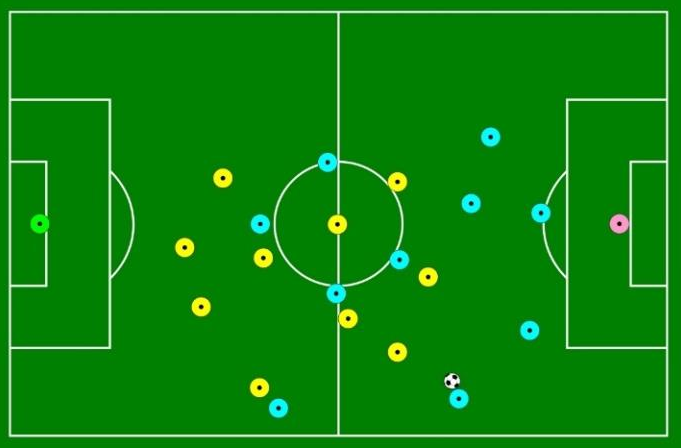
\includegraphics[width=1\linewidth]{figuras/pressing_1a.png}
            \caption{Initial situation}
            \label{fig:pressing_a}
        \end{subfigure}%  
        ~      
        \begin{subfigure}[t]{0.30\textwidth}
            \centering
            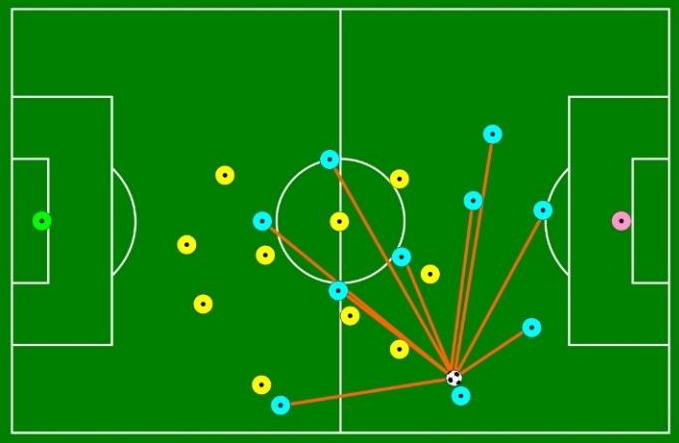
\includegraphics[width=1\linewidth]{figuras/pressing_1b}
            \caption{Possible pass lines}
            \label{fig:pressing_b}
        \end{subfigure}
        ~
        \begin{subfigure}[t]{0.30\textwidth}
            \centering
            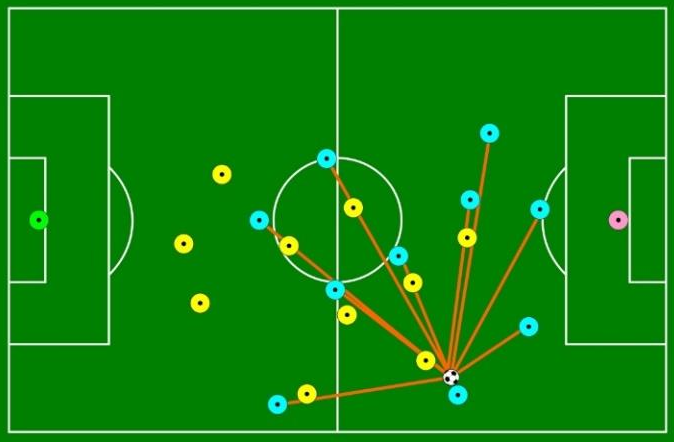
\includegraphics[width=1\linewidth]{figuras/pressing_1c}
            \caption{Pressing in action}
            \label{fig:pressing_c}
        \end{subfigure}%
        
        \caption{Pressing example}
        \label{fig:pressing}
        \end{figure}
    
    \end{frame}

    \begin{frame}{Quer trabalhar só com itemize}
    
        \begin{block}{taqui um exemplo}
            \begin{itemize}
            \item item 1;
            \item item 2;
            \item item 3;
            \item item 4;
            \item item 5.
        \end{itemize}
     \end{block}
    \end{frame}


    \begin{frame}{Ou Equações}
        
        \begin{block}{Pass equation}
            \begin{equation*}\label{eq:f_pass_geral}
            \begin{aligned}
            \operatorname{f_{Pass}}(A, p(i,t), R) = (
            &\operatorname{f_{RadiusAction}}(p(i,t), R) + \\
            &\operatorname{f_{VisionLine}}(A,p(i,t),R)  + \\
            &\operatorname{f_{AdverRadius}}(A,p(i,t))   + \\
            &\operatorname{f_{TeamRadius}}(p(i,t))      +\\
            &\operatorname{f_{Colission}}(A, p(i,t))    + \\
            &\operatorname{f_{InvasionGoalArea}}(p(i,t))
            )
            \end{aligned}
            \end{equation*}
        \end{block}
        
        
        \begin{block}{Block Pass Equation}
    
            \begin{equation*}\label{eq:f_block_pass_geral}
                \begin{aligned}
                \operatorname{f_{BlockPass}}(A, p(i,t), R) =& \operatorname{f_{MinDistance}}(A, p(i,t))
                 +&\operatorname{f_{RadiusAction}}(p(i,t), R) + 
                \\
                & \operatorname{f_{VisionLine}}(A,p(i,t),R) + 
                &\operatorname{f_{AdverRadius}}(A,p(i,t)) + 
                \\
                & \operatorname{f_{TeamRadius}}(p(i,t)) +
                 & \operatorname{f_{Colission}}(A, p(i,t)) + 
                 \\
                & \operatorname{f_{InvasionGoalArea}}(p(i,t))
                \end{aligned}
                \end{equation*}
    
        \end{block}
    \end{frame}


    \begin{frame}{Experiments}
        \begin{block}{Two types of experiment}
           \begin{itemize}
               \item  grSim simulator, the ball and the opponent's robots were positioned differently for visual verification of the behavior of the team robots.
               \item Five soccer matches from league at RoboCup 2019 were selected. From these games, all indirect free kick plays were analyzed.
           \end{itemize}
        \end{block}
    
        \begin{figure}[h]
        \centering
        \begin{adjustbox}{width=.45\textwidth}
            \begin{tikzpicture}[framed]
            \begin{axis}[
            ybar, axis on top,
            title={Increased Success},
            height=7cm, width=\textwidth,
            bar width=0.5cm,
            ymajorgrids, tick align=inside,
            major grid style={draw=white},
            enlarge y limits={value=0,upper},
            ymin=0, ymax=100,
            axis x line*=bottom,
            axis y line*=right,
            y axis line style={opacity=0},
            tickwidth=10pt,
            enlarge x limits=true, scale=1,
            legend style={
                at={(0.5,-0.2)},
                anchor=north,
                legend columns=-1,
                /tikz/every even column/.append style={column sep=0.5cm}
            },
            ylabel={Percentage (\%)},
            symbolic x coords={
                Match 1,Match 2,Match 3, Match 4, Match 5},
            xtick=data,
            nodes near coords={
                \pgfmathprintnumber[precision=1]{\pgfplotspointmeta}
            }
            ]
            \addplot [draw=none, fill=blue!30] coordinates {
                (Match 1,46.23)
                (Match 2,49.57) 
                (Match 3,51.12)
                (Match 4,57.23) 
                (Match 5,65.43) };
            
            
            \addplot [draw=none, fill=green!30] coordinates {
                (Match 1,53.77)
                (Match 2,50.43) 
                (Match 3,48.88)
                (Match 4,42.77) 
                (Match 5,34.57) };
            
            \addplot [draw=none, fill=red!50] coordinates {
                (Match 1,66.11)
                (Match 2,69.31) 
                (Match 3,61.25)
                (Match 4,67.11) 
                (Match 5,69.67) };
            
            \addplot [draw=none, fill=gray!70] coordinates {
                (Match 1,73.30)
                (Match 2,70.21) 
                (Match 3,78.19)
                (Match 4,72.77) 
                (Match 5,74.19) };            
            
            \legend{Original Pass, Original Block Pass, Improved Pass, Improved Block Pass}
            \end{axis}
            \end{tikzpicture}
            \end{adjustbox}
            \caption{Increased percentage success in five RoboCup 2019 matches, with $\approxtext{match} 15-20$ indirect kicks and 10,000 simulations.}
            \label{fig:match}
            \end{figure}
    
    \end{frame}


    \begin{frame}{Figura solta?}
        \begin{figure}[ht]
        \centering
        \begin{adjustbox}{width=.40\linewidth}
            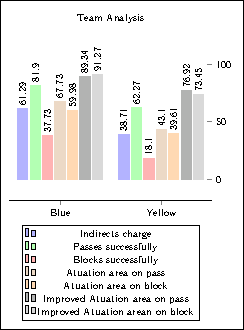
\includegraphics{grafico_team}
        \end{adjustbox}
        \caption{Analysis of two RoboCup 2019 matches with 14 indirect kicks.}
        \label{fig:analysis_match}
        \end{figure}   
    \end{frame}


\begin{frame}
    \frametitle{Tecnologia gera dependência}
    \framesubtitle{E nós somos os viciados!!}
    
    \begin{columns}
        \column{.5\textwidth}
        
        \center{\textcolor{red}{ANTES}}
        \begin{block}{Redes de computadores}
            Compartilhamento de recursos e informações.
        \end{block}     
        
        \begin{block}{Evolução da Internet}
            Pesquisa.
        \end{block}
        
        \column{.5\textwidth}
        \center{\textcolor{red}{DEPOIS}}
        \begin{block}{Redes de computadores}
            Vamos jogar Counter-strike ??
        \end{block}     
        
        \begin{block}{Evolução da Internet}
            Facebook, Torrent, MSN.
        \end{block}
        
    \end{columns}
    
    \begin{alertblock}{Ser-humano e sua criatividade}
        Criatividade é \textcolor{green}{inventar}, experimentar, crescer, \textcolor{red}{correr riscos}, \textcolor{violet}{quebrar regras}, 
        \textcolor{blue}{cometer erros}, e se divertir. (Mary Lou Cook)
    \end{alertblock}
\end{frame}


\begin{frame}
    \frametitle{Coluna com bloco e imagem}
    
    \begin{columns}
        
        \column{.35\textwidth}
        \center
        \begin{block}{\center{destaque}}
            \begin{itemize}
                \item item 1;
                \item item 2;
                \item item 3;
                \item item 4.
            \end{itemize}     
        \end{block} 
        
        \column{.65\textwidth}
        \begin{center}
            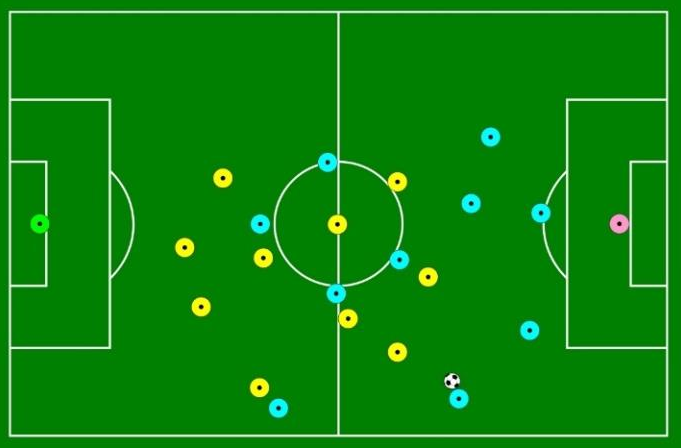
\includegraphics[width=1\textwidth]{figuras/pressing_1a.png} 
        \end{center}
    \end{columns}
\end{frame}


\begin{frame}{Quer brincar com cores dos blocos}
    \begin{exemplo_red}{Exemplo em vermelho}
        bla bla bal
    \end{exemplo_red}

    \begin{exemplo_blue}{Exemplo em azul}
        bla bla bla
    \end{exemplo_blue}


    \begin{block}{Personalize seus blocks se quiser}
        vejas definições no arquivo beamerthefei.sty e acrescente as suas...
        depois compartilha com o pessoal (peça autorização para subir no github)
    \end{block}

\end{frame}
   
\begin{frame}{Brinque a vontade - bloco dentro de bloco}
    \begin{exemplo_red}{Exemplo em vermelho}
        bla bla bla
        \begin{exemplo_blue}{Exemplo em azul}
            bla bla bla
        \end{exemplo_blue}
    \end{exemplo_red}
    
\end{frame}

\begin{frame}{Blocos com sombra}
    
    \begin{exemplo_red_shadow}{Título como parâmetro}
    {Texto também deve estar entre chaves}
    \end{exemplo_red_shadow}

    \begin{exemplo_blue_shadow}{Título como parâmetro}
    {Texto também deve estar entre chaves}
    \end{exemplo_blue_shadow}

\end{frame}

\end{document}
